\documentclass[ngerman]{gdb-aufgabenblatt}


\renewcommand{\Aufgabenblatt}{5}
\renewcommand{\Ausgabedatum}{Mi. 09.12.2015}
\renewcommand{\Abgabedatum}{Do. 08.01.2016}
\renewcommand{\Gruppe}{Kraemer, Mirzada, Frangopoulos, Heid}
\renewcommand{\STiNEGruppe}{06}
\renewcommand{\Semester}{WS 2015/16}


\begin{document}


\section*{Aufgabe 1: Referentielle Aktionen}
\subsection*{a) Anforderungen an sicheres Schema}
Das Ergebnis der referentiellen Aktionen darf nicht von der Reihenfolge der Ausf�hrung dieser abh�ngig sein.

\subsection*{b) Referenzgraph}
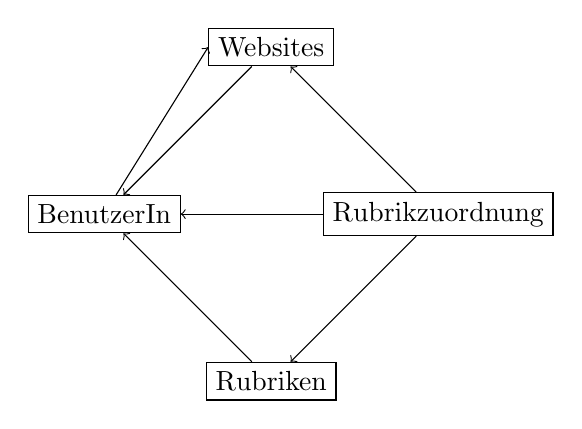
\begin{tikzpicture}[->, node distance=3cm]
\node[draw] (Websites) at (0,0) {Websites};
\node[draw] (BenutzerIn) [below left of= Websites] {BenutzerIn};
\node[draw] (Rubrikzuordnung) [below right of= Websites] {Rubrikzuordnung};
\node[draw] (Rubriken) [below right of= BenutzerIn] {Rubriken};

\draw[->] (Websites) 		-- (BenutzerIn);
\draw[->] (Rubrikzuordnung) -- (BenutzerIn);
\draw[->] (Rubriken) 		-- (BenutzerIn);
\draw[->] (BenutzerIn) 		-- (Websites.west);
\draw[->] (Rubrikzuordnung) -- (Websites);
\draw[->] (Rubrikzuordnung) -- (Rubriken);


\end{tikzpicture}

\subsection*{c) Unsicherheit}
Beim L�schen eines Eintrags aus BenutzerIn gibt es 2 unterschiedliche m�gliche Effekte auf die Eintr�ge von Rubrikzuordnung.\\
Das L�schen k�nnte auf direktem Weg kaskadieren oder per indirektem Weg �ber Rubriken verboten werden und so unterschiedliche Ergebnisse erzielt werden, was das Schema unsicher macht.

\subsection*{d) Vorkehrungen}
Referenz auf BenutzerIn von Rubrikzuordnung : On Delete CASCADE -> On Delete RESTRICT

\newpage
\section*{Aufgabe 2: �nderbarkeit von Sichten}

\subsection*{Sichterstellung}
\subsubsection*{i) Enterprise-Crew}
\begin{verbatim}
CREATE VIEW EnterpriseCrew AS
    SELECT b.BNr, b.Name, b.Rang
    FROM Raumschiffe r, Besatzungsmitglieder b
    WHERE b.Schiff = r.RNr
    AND r.Name = 'Enterprise';
		
Die Sicht ist nicht �nderbar, da hier Tabellen verbunden werden.
\end{verbatim}

\subsubsection*{ii) Captains}
\begin{verbatim}
CREATE VIEW Captains AS
    SELECT Name
    FROM Besatzungsmitglieder
    WHERE Rang = 'Captain';
		
Auch hier ist die Sicht nicht �nderbar, doch diesmal aus dem Grund,
dass sie nicht den Prim�rschl�ssel der referenzierten Besatzungsmitglieder-
Relation enth�lt.
\end{verbatim}

\subsubsection*{iii) WarpFed}
\begin{verbatim}
CREATE VIEW WarpFed AS
    SELECT RNr, Fraktion, Baujahr
    FROM Raumschiffe
    WHERE Geschwindigkeit >= 1
    AND Fraktion = 'F�rderation';

Diesmal ist die Sicht �nderbar.
\end{verbatim}

\subsection*{b) �nderbarkeit}
\begin{tabular}{|c|l|}
\hline
i)&Es handelt sich um eine erlaubte Operation.\\
\hline
ii)& Es handelt sich um eine nicht erlaubte Operation, da das Schiff nicht zur F�rderation geh�rt.\\
\hline
iii)& Es handelt sich um eine erlaubte Operation.\\
\hline
iv)& Es handelt sich um eine Operation, die zur�ckgewiesen wird.\\
\hline
v)& Es handelt sich um eine erlaubte Operation, das Tupel taucht jedoch nicht in der Sicht auf.\\
\hline
\end{tabular}

\section*{Aufgabe 3: Serialisierbarkeit und Anomalien}
\subsection*{a) Belegungen}
\begin{tabular}{|c|c|c|c|c|c|c|}
\hline
&$S_1$&$S_2$&$S_3$&$S_4$&$S_5$&$S_6$\\
\hline
$A$&$305$&$195$&$300$&$190$&$115$&$300$\\
\hline
$B$&$195$&$5$&$5$&$5$&$5$&$5$\\
\hline
\end{tabular}
\subsection*{b) Abh�ngigkeiten}

\begin{tabular}{|c|l|}
\hline
$S_1$&Die Operation $r_2(A)$ ist abh�ngig von Operation $w_1(A)$.\\
\hline
$S_2$&Hier sind keine Operationen voneinander abh�ngig.\\
\hline
$S_3$&Die Operation $r_1(B)$ ist von der Operation $w_2(B)$ und die Operation $r_1(A)$ von der Operation $w_2(A)$ abh�ngig.\\
\hline
$S_4$&Die Operation $r_1(B)$ ist von der Operation $w_2(B)$ abh�ngig.\\
\hline
$S_5$&Hier sind keine Operationen voneinander abh�ngig.\\
\hline
$S_6$&Die Operation $r_1(B)$ ist von der Operation $w_2(B)$ und die Operation $r_1(A)$ von der Operation $w_2(A)$ abh�ngig.\\
\hline
\end{tabular}

\subsection*{c) Serialisierbarkeit}
\begin{tabular}{|c|l|}
\hline
$S_1$&Der Schedule ist seriell. $T_1$ wird vor $T_2$ ausgef�hrt.\\
\hline
$S_2$&Der Schedule ist nicht serialisierbar, da bei einer Nacheinanderausf�hrung der \\
&Transaktionen bestimmte Leseoperationen abh�ngig von vorher geschehenen\\
&Schreiboperationen w�ren. Dies ist bei $S_2$ nicht der Fall.\\
\hline
$S_3$&Der Schedule ist serialisierbar. Es wird nach der Serialisierung $T_2$ vor $T_1$ ausgef�hrt.\\
\hline
$S_4$&Der Schedule ist nicht serialisierbar.\\
\hline
$S_5$&Der Schedule ist nicht serialisierbar, da bei einer Nacheinanderausf�hrung der \\
&Transaktionen bestimmte Leseoperationen abh�ngig von vorher geschehenen \\
&Schreiboperationen w�ren. Dies ist bei $S_5$ nicht der Fall.\\
\hline
$S_6$&Der Schedule ist seriell. Es wird $T_2$ vor $T_1$ ausgef�hrt.\\
\hline
\end{tabular}

\newpage
\section*{Aufgabe 4: Transaktionen}

\begin{tabular}{|p{2cm}|p{2cm}|p{2cm}|p{2cm}|p{1cm}|p{1cm}|p{1cm}|p{3cm}|}
\hline
Zeitschritt & T\ts{1} & T\ts{2} & T\ts{3} & x & y & z & Bemerkung\\
\hline
\hline
0 &  &  &  & NL & NL & NL & \\
\hline
1 & lock(x,X) 	&  			&  			& X\ts{1} & NL 		& NL & \\
\hline
2 & write(x) 	& lock(y,R) &  			& X\ts{1} & R\ts{2} & NL & \\
\hline
3 &  			& read(y)	& lock(z,R) & X\ts{1} & R\ts{2} & R\ts{3} & \\
\hline
4 &  			&  			& read(z)	& X\ts{1} & R\ts{2} & R\ts{3} & \\
\hline
5 &  			&  			& lock(y,X) & X\ts{1} & R\ts{2} & R\ts{3} & Warten auf Freigabe von y \\
\hline
6 &  			& lock(z,R) &  			& X\ts{1} & R\ts{2} & R\ts{2,3} & \\
\hline
7 & lock(z,X)	& read(z) 	& 			& X\ts{1} & R\ts{2} & R\ts{2,3} & Warten auf Freigabe von z \\
\hline
8 & 			& read(y) 	&  			& X\ts{1} & R\ts{2} & R\ts{2,3} & \\
\hline
9 &  			& unlock(y) &  			& X\ts{1} & X\ts{3} & R\ts{2,3} & Melden an T\ts{3}\\
\hline
10 &  			& unlock(z) & write(y)	& X\ts{1} & X\ts{3} & R\ts{3} & \\
\hline
11 &  			& commit 	& lock(z,X)	& X\ts{1} & X\ts{3} & R\ts{3} & \\
\hline
12 &  			&  			& write(z) 	& X\ts{1} & X\ts{3} & R\ts{3} & \\
\hline
13 &  			&  			& unlock(y) & X\ts{1} & NL & R\ts{3} & \\
\hline
14 &  			& 			& unlock(z) & X\ts{1} & NL & X\ts{1} & Melden an T\ts{1} \\
\hline
15 & write(z)	&  			& commit	& X\ts{1} & NL & X\ts{1} & \\
\hline
16 & unlock(x)	&  			&  			& NL & NL & X\ts{1} & \\
\hline
17 & unlock(z)	&  			&  			& NL & NL & NL & \\
\hline
18 & commit		&  			&  			& NL & NL & NL & \\
\hline
\end{tabular}

\end{document}